\documentclass{book}
\usepackage[utf8]{inputenc}
\usepackage[spanish]{babel}
\usepackage{graphicx}
\usepackage{graphicx,subfig}
\usepackage{mathptmx}
\usepackage{multicol}
\usepackage{color}
\usepackage{listings}
\usepackage[usenames,dvipsnames,svgnames,table]{xcolor}

\begin{document}
	\thispagestyle{empty}
	\frontmatter
	
	\section*{TÍTULO}
	\Large{Diseño e implementación de un entorno computacional para la ayuda en la síntesis de sonidos musicales}
	\section*{OBJETIVOS}
	\begin{itemize}
		\item Construcción de una interfaz de usuario para la ayuda visual y auditiva en la composición y síntesis de sonidos.
		\item Implementación del los modelos generados en otros ambientes de software.
	\end{itemize}
	\section*{DEFINICIÓN DEL PROBLEMA}
	La propuesta hoy presentada comenzó como una necesidad no resuelta por las herramientas disponibles y demandas hechas por los proyectos de escasos recursos presupuestarios y personal, mejor conocidos como proyectos independientes en los ámbitos de producción en software destinados a la recreación y el ocio como lo son juegos de video y multimedia, a su vez, disponer de una herramienta adicional a los ya indispensables usos del procesador de textos, hojas de cálculo, controlador de diapositivas, entre otros integrados y dependientes exclusivamente del equipo de cómputo. \par
	
	Si bien, este proyecto no es pionero en su finalidad, en lo que a producción de origen totalmente computacional es referido, la composición de obras auditivas en formatos digitales sigue siendo parcialmente dependiente de la captura y edición de la información proveniente de los instrumentos musicales físicos capturados por periféricos especializados, donde en estos se requiere un compromiso absoluto en la disciplina artística, así como la ingeniería propia involucrada en el muestreo y alteración en las señales de audio.\pagebreak\par
	
	Existen algunas herramientas de porte comercial dedicadas a la generación del audio sin la demanda de un instrumento o captura de este, aun así, estas no ha sido diseñadas en dotar a su producto de una calidad definitiva, pues ha sido concebida como una referencia o prueba de concepto, pues el método de producción basado en la adición estratégica con muestras pre-grabadas de notas musicales, tienen una clara limitante en cuanto a tiempo, diversidad en variaciones de interpretación entre muchos aspectos no deseados en vista a un producto final, pues a nivel de consumidor, no sería de su agrado la escucha de sonidos tan parecidos y sin sus variaciones.\par
	
	Esta problemática no refiere a una urgencia en el mercado, aunque si aspira a la dar un nuevo abanico de opciones en cuanto la producción musical, una que permita cubrir la sincronización con el tiempo así como la correcta interpretación de sonidos hechos en instrumentos musicales, en otras palabras, dar a los compositores sean aspirantes o expertos la posibilidad de aumentar e inaugurar una mayor y más eficiente producción, brindando las bondades que nos ha traído la programación informática, referentes al propio soporte, el trabajo re-utilizable incluso en cuanto a un nuevo paradigma de almacenamiento y respuesta computacional adecuada a los temas sonoros.\par
	
	Véase un anuncio publicitario compuesto con los \emph{jingles} establecidos de la corporación, el repertorio cultural en potencia al disponer a cada usuario las herramientas para componer la futura obra maestra en una industria saturada por el monopolio de tendencias actuales, surgidas en culturas y lugares distintos, todo disponible desde la misma plataforma y capacidades de la máquina capaz de ejecutar un editor de textos comercial.\par
	
	Después de todo, ya existen los conjuntos de herramientas totalmente independientes para la elaboración de sus respectivos productos, hablando también de aquellos más complejos como obras audiovisuales, construcción de modelos en tres dimensiones o combinando todos estos para la elaboración de aplicaciones gráficas orientadas al entretenimiento, mejor conocidos como \emph{videojuegos}\par
	
	\pagebreak
	\section*{MÉTODO}
	La siguiente imagen muestra una representación simplificada sobre la propuesta de solución al completo, donde se tiene planeadas todas sus funcionalidades y operaciones al menos de cara a un lanzamiento hacia el público interesado, más no uno comercial.\par
	
	Cabe aclarar, este proyecto comprende más objetivos y características para resolver las problemáticas anteriormente planteadas. Aunque por los alcances limitados en tiempo, recursos y personal, se ha decidido centrar los esfuerzos en la parte más significativa en la solución de software, siendo el módulo \emph{Tuner}.
	\begin{figure}[h]
		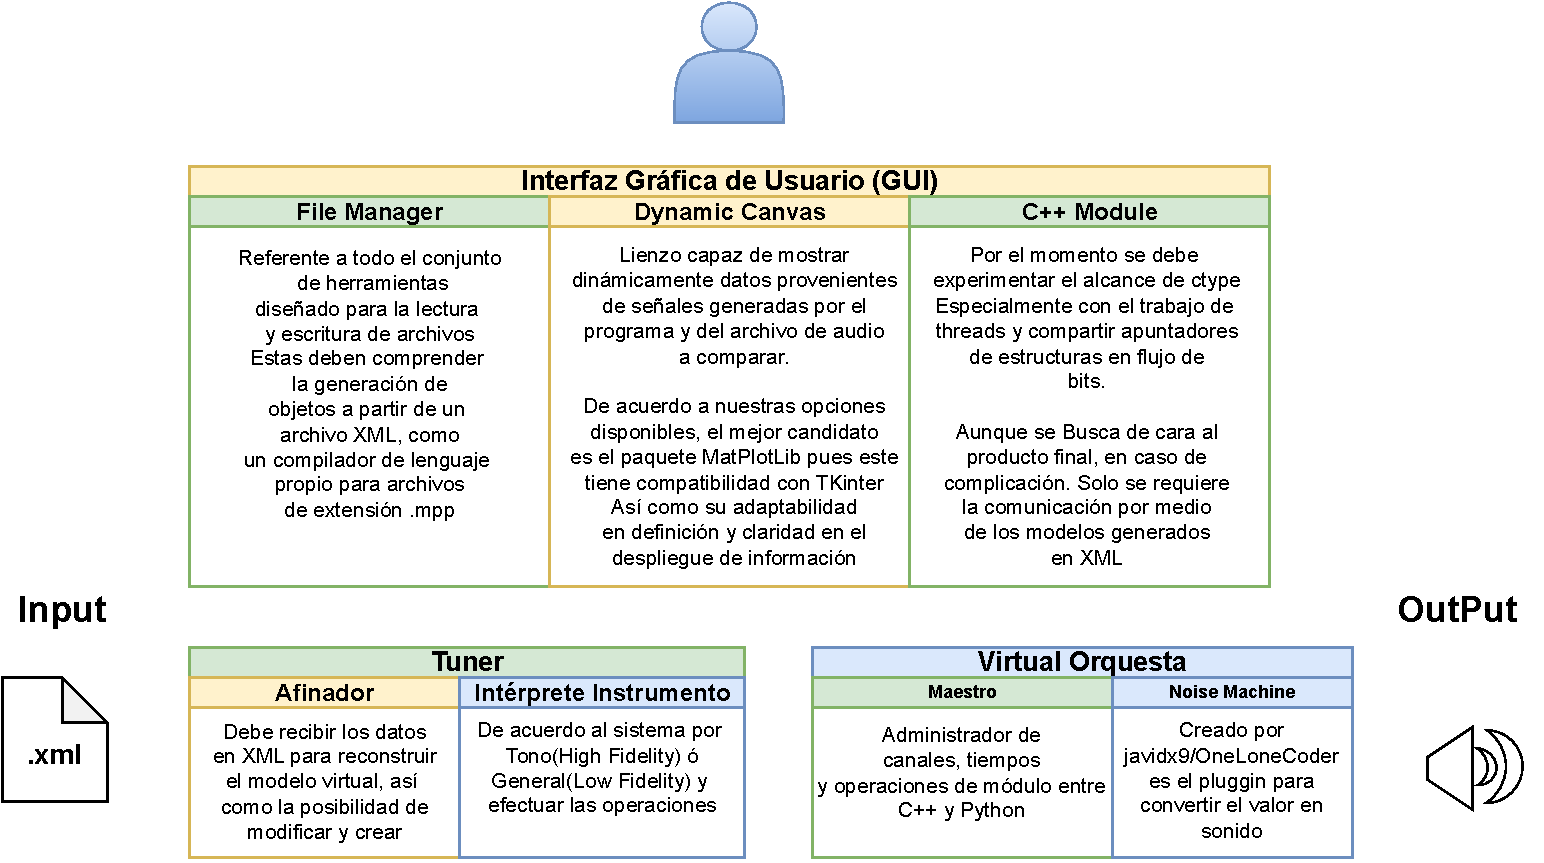
\includegraphics[width=1.25\linewidth]{../Assets/images/musiC++_Diagram_cut}
		\caption{ Diagrama General del Proyecto}
	\end{figure} 
	
	\pagebreak
	Profundizando en los módulos mostrados anteriormente:
	\subsection*{Interfaz Gráfica de Usuario (GUI)}
	El enfoque comercial del proyecto, exige que este contenga por lo menos una visualización cercana a los estándares en herramientas de software, si bien, el público general cambia su tendencia en cuanto conocimientos informáticos básicos, sería un error cerrarnos de cara a una presentación como la manipulación para una terminal de consola. Se ha experimentado construir una GUI con el lenguaje \emph{C++}, sin embargo no pudo encontrarse una biblioteca adecuada, mucho menos un resultado satisfactorio para delegar todo el proyecto a un único lenguaje de programación, por lo tanto, se trabajará con Python en el \emph{FrontEnd}, es decir, todo contacto con el usuario final.\par
	\subsection*{File Manager}
	Ya que nuestro propósito es la generación de archivos cuya información pueda interpretarse por un estándar orientado a audio, así como la preservación del trabajo en un lenguaje de programación, es imperativo usar varios sistemas de lectura y escritura de archivos en ambos lenguajes a utilizar, siendo \emph{Python} y \emph{C++}, estos contienen una biblioteca en sus paquetes fundamentales, siendo la función \emph{open} y \emph{fstream} respectivamente. Por otra parte, se necesitará de una biblioteca especializada en convertir la información de un texto etiquetado como lo es el formato XML. No solo es un estándar que permite escalar las funciones del proyecto a futuro con otros productos de software, sino que al ser un formato simple y en cierto punto, indicativo para ser editado manualmente.
	\subsection*{Dynamic Canvas}
	Si bien, esta parte podría únicamente ser útil en lo que respecta la construcción del módulo afinador. Puede utilizarse en tiempo real la representación gráfica de la información generada, desde los armónicos que participan en la mezcla del sonido, una visión más amigable de cara al usuario de los eventos programados, entre otras cosas. Ya que esto está ligado a la GUI así como el afinador, su desarrollo sería exclusivamente en Python, optando por la opción que ofrece el paquete de \emph{MatPlotLib} por su compatibilidad con \emph{TKinter}.
	\subsection*{C/C++ Module}
	Debido a las características por implementar, es conveniente dejar a Python como aquel que tenga el ejecutable inicial, así como ser el eje de las herramientas que conlleve el proyecto. Este ofrece una opción denominada como \emph{ctype} el cual permite convocar código en \emph{C/C++} colocando y devolviendo datos primitivos, aún no se ha experimentado del todo, pues se requiere de la certeza y técnicas en cuanto el envío de apuntadores para arreglos de datos, estructuras específicas así como su correcto funcionamiento con múltiples hilos de ejecución.
	\subsection*{Tuner}
	Este módulo deberá ser construido en casi su totalidad en lenguaje \emph{Python} pues al comparar en tiempo real la generación de señales, este deberá sumergirse por completo en el ambiente, aunque algunas partes podrían invocarse desde \emph{C/C++} si la eficiencia es significativa. Por otra parte, debe cumplir al menos con la reproducción del modelo concurrente. Así como la lectura de información auditiva escrita en un archivo \emph{.wav} para su comparación ante el modelo generado. 
	\subsection*{Generador de Señales}
	Siendo la parte más visual del proyecto, esta tiene que generar señales con los datos otorgados por el usuario, con representación gráfica en tiempo contra amplitud, frecuencia contra amplitud, frecuencia contra tiempo, en cualquiera pueda ser la información necesaria para la correcta implementación de valores en los modelos matemáticos. Así como la designación de al menos un método de aproximación en comparación a las muestras de audio.
	\subsection*{Virtual Instrument}
	Siendo una convención escrita sobre las reglas del lenguaje de etiquetado XML, es una designación simple y comprensible para la re-construcción de los valores del audio. Consistiendo en 2 secciones, siendo el método, una colección de modelos trigonométricos y una plantilla de señal, siendo una representación de convertir la señal digital absoluta en una transaccional analógica, como lo son las señales musicales en la práctica. 
	\pagebreak\subsection*{Virtual Orquesta}
	Este es un módulo enfocado al procesamiento central de la información, pues estará diseñado para invocar la interpretación de las instrucciones y ajustes dados por el usuario, administración de los múltiples hilos dedicados, pausa, reinicio, incluso a la captura en tiempo real de notas generadas por el usuario mediante una entrada estándar así como la posibilidad de escalar a un instrumento especializado.
	\subsection*{MasterChord}
	Siendo esta parte administrativa, deberá cumplir con una facilidad de funciones que puedan ser citadas como servicios desde la GUI así como la respuesta de información siendo instrumentos, posición de notas, tiempo real o cualquier información correspondiente a una visualización con propósitos artísticos o técnicos. Si bien las funciones gráficas son prescindibles, se deja abierta la posibilidad de escalar al producto final.
	\subsection*{NoiseMachine}
	Esta es una cabecera hecha por \emph{Javidx9/OneLoneCoder} que nos permite la comunicación con el hardware hecho para la reproducción de audio mediante la solicitud del tiempo en valor de la amplitud otorgado por una función asignada. Esta pieza limita el proyecto a plataformas con sistema operativo Windows 7 en adelante, con compatibilidad para arquitectura de x32 bits.
	\section*{INVENTARIO DE ASIGNATURAS INVOLUCRADAS}
	Correspondientes al plan de estudios de Ingeniería en Computación(2016)
	\begin{itemize}
		\item Álgebra/Álgebra Lineal
		\item Fundamentos de Física/Programación
		\item Estructuras de datos y algoritmos I/II/Discretas
		\item Cálculo y Geometría Analítica/Integral
		\item Ecuaciones Diferenciales/ Matemáticas Avanzadas
		\item Señales y Sistemas/ Sistemas de Comunicaciones
	\end{itemize}
	\pagebreak\section*{ÍNDICE DESGLOSADO}
	\renewcommand{\theenumii}{\arabic{enumii}}
	\begin{enumerate}
		\item Introducción
		\begin{enumerate}
			\item Objetivo
			\item Planteamiento del problema
			\item Estado del Arte
			\item Fundamentos de la organización Musical
		\end{enumerate}
		\item Análisis y Procesamiento de Audio
		\begin{enumerate}
			\item Definición Técnica del Audio
			\item Captura de Información
			\item Procesamiento de Señal
			\item Métodos de aproximación
		\end{enumerate}
		\item Construcción de la NoiseMachine
		\begin{enumerate}
			\item Estudio del proyecto olcSynth
			\item Aporte de propuesta
			\item Cambios y pruebas del software
			\item Implementación y Proyección a Futuro
		\end{enumerate}
		\item Construcción del Tunner
		\begin{enumerate}
			\item Estrategia y Diseño
			\item Manejo de excepciones
			\item Capacidades mínimas
			\item Áreas de Innovación
		\end{enumerate}
		\item Diseño de los Instrumentos Virtuales
		\begin{enumerate}
			\item Resumen de XML
			\item Propuesta de Convención
			\item Proyecciones con musiC++
			\item Comparación contra formatos estandarizados
		\end{enumerate}
		\pagebreak\item Guía de Usuario
		\begin{enumerate}
			\item Paso 1: Recolección de Muestra
			\item Paso 2: Afinar el Instrumento Virtual
			\item Paso 3: Prueba de Sonido
			\item Paso 4: Exportación a otros Productos
		\end{enumerate}
		\item Conclusiones
		\item Bibliografía
		\item Anexos
	\end{enumerate}
	\section*{RESULTADOS ESPERADOS}
	Con el entorno de producción finalizado, se espera obtener en referencia al producto, como en propuesta de uso:
	\begin{itemize}
		\item Nuevo Formato de Almacenamiento de información orientado al arte musical
		\item Modelos Instrumentales digitales utilizables en otros proyectos de programación
		\item Facilidad en su comprensión para el usuario en su fabricación de Instrumentos virtuales
		\item Simulación de instrumental precisa y universal
		\item Diseño escalable al número de funciones y modos de interpretación del sonido producido
		\item Independencia de periféricos instrumentales reales
	\end{itemize}
	Adicionalmente, se ha hablado en ocasiones del alcance sobre este proyecto, pues proviene de otra propuesta para la generación musical, siendo esta por medio de la programación en un lenguaje especializado en la logística de información en lo que respecta el tiempo, por otra parte, una cercanía con los estándares del lenguaje musical. De esta manera, se espera un uso complementario en programas destinados al ocio y confort del usuario final referente a la conocida \emph{experiencia} en este tipo de entornos.\par
	
	Citando un ejemplo más específico, en la industria del entretenimiento digital como lo son los videojuegos, entornos virtuales variables sujetos a la interacción usuario computadora, donde gracias a esta propuesta se podría brindar una experiencia sonora artística mucho más apta y factible. Un alto punto de valor agregado que puede significar muchas más ganancias, prestigio y un nuevo paradigma.\par
	
	\section*{CRONOGRAMA}
	\begin{figure}[h]
		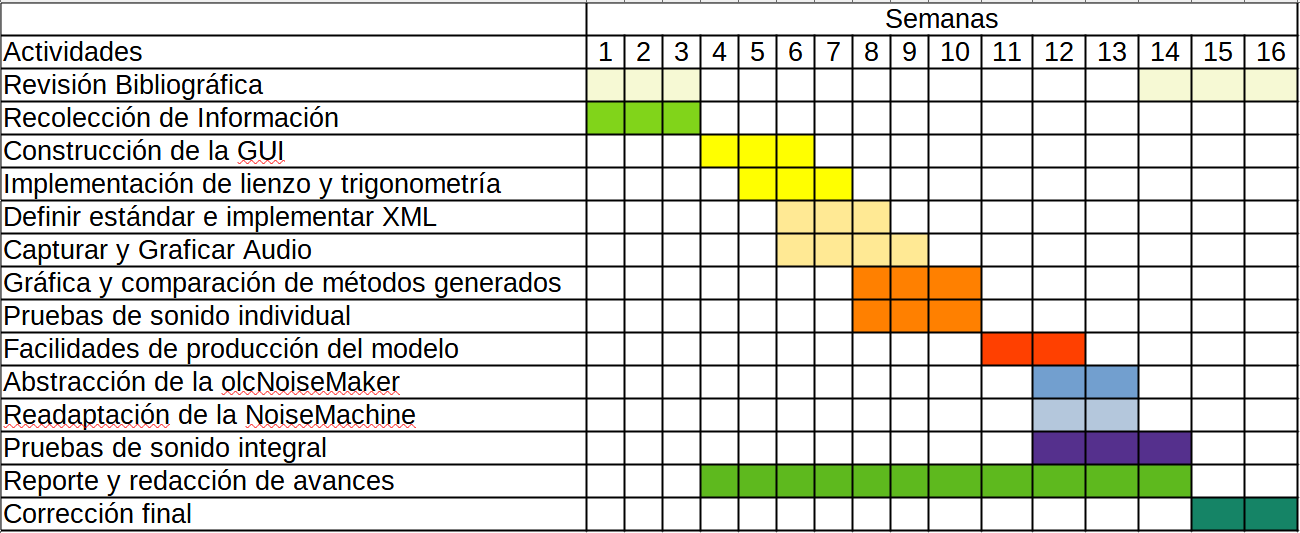
\includegraphics[width=\linewidth]{../Assets/images/cronograma}
		\caption{Planeación estimada del desarrollo}
	\end{figure} 
\end{document}

